\begin{frame}[t]{Structuredness of a formula}
	\begin{itemize}[<+->]
		\item Let $\varphi$ be a DNNF formula and let $V := \mathrm{VAR}(\varphi)$.
		\item A \textbf{$\mathbf{v}$Tree} $T$ is a binary tree where the leaves of the tree has a one-to-one correspondence to the variables of $\varphi$.
		\item The formula $\varphi$ respects $T$ if and only if for each subformula of  $\varphi$ of the form $\varphi' := \psi_1 \land \psi_2$, there is a vertex $v \in V(T)$ with two children $v_1, v_2$, where $\mathrm{VAR}(\psi_1)\subseteq V(T_{v_1})$ and $\mathrm{VAR}(\psi_2) \subseteq V(T_{v_2})$, where $T_v$ is the subtree of $T$ rooted at $v$. We say $\varphi'$ respects $v$ in this case.
		\item A formula $\varphi$ is structured, if there is a $v$tree $T$ over the vertices of $\varphi$, such that $\varphi$ respects $T$.
	\end{itemize}

	\uncover<3->{
	\begin{minipage}{.49\linewidth}
		$$(x\land(y\lor z)) \lor (z \textcolor{red}{\bm{\land}} \lnot x)$$
	\end{minipage}
	\hfill
	\begin{minipage}{.49\linewidth}
		\centering
		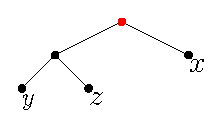
\includegraphics[width=.6\linewidth]{figures/vtree.eps}
	\end{minipage}
	}
\end{frame}

\begin{frame}[t]{Incidence graphs and structure of formulas}
	\begin{itemize}
		\item The \textbf{incidence graph} of $\mathcal{H}$ is a 
		\item[] \hspace{1cm}bipartite graph $(V(\mathcal{H}) \cup E(\mathcal{H}), E)$
		\item[] \hspace{1cm},where $\{v, e\} \in E$ iff $v \in e$.
			\vspace{.5cm}
		\uncover<2->{\item Hypergraph of a CNF-Formula.}
		\uncover<3->{\item The incidence graph of a CNF-Formula is
		\item[] \hspace {1cm} the incidence graph of its hyper graph.}
		\uncover<4->{\item A CNF-Formula is $\beta$-acyclic if its hypergraph is.}

		\item {}[todo] MIM-width
		\item []example on the board.
	\end{itemize}

\end{frame}
